\documentclass[11pt,a4paper]{article}

\usepackage{polski}
\usepackage[utf8]{inputenc}
\usepackage{hyperref}
\usepackage{graphicx}

\setcounter{tocdepth}{3}

\title{Bitcoin Excavator - Dokumentacja}
\author{Michał Szczygieł \and Aleksander Śmierciak}
\date{Wrzesień 2014}

\begin{document}
\maketitle

\tableofcontents

\section{Wstęp}

Niniejszy dokument opisuje projekt oprogramowania wydobywającego jednostki kryptowaluty Bitcoin. Projekt ten jest projektem semestralnym z przedmiotu Programowanie równoległe i rozproszone i ma za zadanie zademonstrować zrozumienie studentów w temacie wykorzystania specyfiki kart graficznych w celu wykonywania obliczeń.

\section{Czym jest Bitcoin?}
Jest to kryptowaluta, wprowadzona w 2009 roku przez osobę (bądź grupę osób) o pseudonimie Satoshi Nakamoto. Nazwa odnosi się także do używającego jej otwartoźródłowego oprogramowania oraz sieci peer-to-peer którą formuje. „Bitmonety” mogą zostać zapisane na komputerze osobistym w formie pliku portfela lub być przetrzymywane w prowadzonym przez osoby trzecie zewnętrznym serwisie zajmującym się przechowywaniem takich portfeli. W każdym z tych przypadków Bitcoiny mogą zostać przesłane do innej osoby przez Internet do dowolnego posiadacza adresu bitcoin. Każdy bitcoin dzieli się na 100 000 000 mniejszych jednostek, zwanych czasem satoshi.


\section{Specyfikacja techniczna Bitcoin}

Bitcoin jest implementacją konceptu b-money autorstwa Wei Daia oraz Bitgold autorstwa Nicka Szabo, opartą na sieci P2P. Zasady funkcjonowania systemu są opisane w specyfikacji technicznej stworzonej i opublikowanej w 2008 roku przez Satoshiego Nakamoto.

\subsection{Adresy}

Każda osoba uczestnicząca w sieci bitcoin ma portfel zawierający dowolną liczbę par kluczy kryptograficznych. Klucze publiczne, zwane też adresami bitcoin, działają jako miejsce źródłowe oraz miejsce docelowe dla wszystkich płatności. Odpowiadające im prywatne klucze autoryzują płatności tylko dla posiadającego je użytkownika. Adresy nie zawierają żadnej informacji na temat ich właściciela i są zazwyczaj anonimowe.

Adresy, w łatwej do odczytania przez człowieka formie, są ciągami tekstowymi, składającymi się z liczb i liter o długości około 34 znaków w formie zbliżonej do 1rYK1YzEGa59pI314159KUF2Za4jAYYTd. Rozpoczynają się zawsze od liczby 1 lub 3, zawierają wielkie i małe litery oraz cyfry alfabetu łacińskiego z wykluczeniem: cyfry 0, wielkiej litery O, wielkiej litery I i małej litery l.

Użytkownicy Bitcoina mogą posiadać wiele adresów, a właściwie mogą generować nowe adresy bez żadnych ograniczeń, ponieważ generowanie nowego adresu jest relatywnie natychmiastowe, równe wygenerowaniu nowej pary kluczy prywatnego/publicznego oraz nie wymaga kontaktu z resztą sieci. Jest także wykorzystywany do jednoznacznej identyfikacji zapłaty za towar poprzez tworzenie unikalnego adresu bitcoin dla każdej transakcji, ponieważ obecnie sieć nie dopuszcza tytułu przelewu znanego z tradycyjnych form przekazu. Tworzenie jednorazowych adresów wykorzystywanych do pojedynczego celu może też pomóc w zachowaniu anonimowości użytkownika.

\subsection{Transakcje}

Bitmonety zawierają klucz publiczny (adres) aktualnego posiadacza. Kiedy użytkownik A przetransferuje jakąś ilość do użytkownika B, A rezygnuje z ich posiadania, dodając klucz publiczny (adres) B do tych monet oraz podpisując je własnym kluczem prywatnym. Następnie ogłasza wykonaną przez siebie transakcję w komunikacie wysłanym do sieci peer-to-peer. Reszta sieci sprawdza poprawność zastosowanych w transakcji podpisów cyfrowych oraz ilości monet przed jej zaakceptowaniem.

\subsection{Łańcuch bloków}

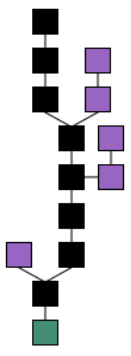
\includegraphics{images/block_chains.PNG}

Główny łańcuch (czarny) składa się z najdłuższej serii bloków poczynając od bloku genezy (zielonego) na aktualnym bloku kończąc. Osierocone bloki (fioletowe) istnieją poza głównym łańcuchem.

Dowolna transakcja rozesłana do innych węzłów nie staje się natychmiastowo „oficjalna”, zanim nie zostanie dodana do i potwierdzona na wspólnie utrzymywanej, oznakowanej znacznikami czasu liście wszystkich znanych transakcji, tj. łańcucha bloków. Potwierdzenie to jest oparte na systemie matematycznych dowodów wykonanych działań, zwanym inaczej „proof of work”, w celu zapobieżenia podwójnemu wydawaniu oraz fałszerstwu.

Bardziej szczegółowo, każdy generujący węzeł (emitent) zbiera wszystkie niepotwierdzone transakcje, które zna w kandydacie na blok – pliku zawierającym między innymi kryptograficzne hashe poprzedniego poprawnego bloku, znanego temu węzłowi. Następnie próbuje obliczyć kryptograficzny hash tego bloku z określonymi cechami, co wymaga z góry przewidywalnej liczby prób i błędów. Kiedy znajdzie rozwiązanie, ogłasza je reszcie sieci. Węzły otrzymujące nowo rozwiązany blok, sprawdzają jego poprawność przed zaakceptowaniem i dodaniem do łańcucha.

Ostatecznie łańcuch bloków zawiera kryptograficzną historię zmian posiadania wszystkich monet, poczynając od adresu ich emitenta aż po adres aktualnego posiadacza. Dlatego właśnie jeżeli użytkownik spróbuje ponownie wykorzystać wydane wcześniej monety, sieć odrzuci próbę wykonania takiej transakcji.

\subsection{Generowanie bitmonet}

Generowanie nowych monet w sieci bitcoin ma charakter probabilistyczny – może na nie trafić każdy użytkownik sieci, aktywnie weryfikujący transakcje po spełnieniu określonego warunku, statystycznie bardzo mało prawdopodobnego. Generowanie bitmonet jest często nazywane „wydobywaniem”, poprzez analogię do wydobywania złota. 

Prawdopodobieństwo, iż dany użytkownik otrzyma partię monet, zależy od stosunku ilości mocy obliczeniowej, wniesionej do sieci za jego pośrednictwem, do sumy mocy obliczeniowej wniesionej przez wszystkie węzły. Liczba bitmonet stworzona w partii nigdy nie jest większa niż 25 BTC (dane na luty 2013), a nagrody są zaprogramowane na zmniejszanie się w czasie aż do zera, tak aby kiedykolwiek mogło zaistnieć nie więcej niż 21 milionów monet. W miarę, jak wypłaty będą się zmniejszać, oczekuje się, iż zbieranie opłat transakcyjnych będzie motywacją dla użytkowników do uruchamiania węzłów generujących.

Wszystkie węzły generujące sieci współzawodniczą w celu bycia pierwszymi w znalezieniu rozwiązania problemu kryptograficznego dla przetwarzanego bloku kandydującego, co wymaga stosowania powtarzających się prób i błędów. Kiedy węzeł znajdzie takie rozwiązanie, ogłasza je reszcie sieci oraz deklaruje się posiadaczem nowej partii bitmonet. Węzły otrzymujące nowo rozwiązany blok sprawdzają jego poprawność przed zaakceptowaniem i dodaniem do łańcucha. Węzły mogą używać CPU, GPU, FPGA oraz ASIC. W praktyce w 2013 roku wszystkie liczące się „kopalnie” korzystają ze specjalizowanych układów ASIC. Użytkownicy mogą także generować bitmonety grupowo.

Każdy blok jest generowany co średnio 10 minut, każdy węzeł osobno co 2016 bloków (co w praktyce zajmuje średnio 2 tygodnie) rekalkuluje stopień trudności problemu, który próbuje rozwiązać, używając do tego średniej kroczącej, celującej w średnią liczbę bloków na godzinę. Jeżeli bloki są generowane zbyt szybko lub zbyt wolno, co zależy od zwiększającej lub zmniejszającej się mocy obliczeniowej całej sieci, stopień trudności odpowiednio wzrasta lub maleje.

\subsection{Opłaty transakcyjne}

Ponieważ węzły nie mają obowiązku zawierać transakcji w blokach, które generują, wysyłający transfery pieniężne za pomocą Bitcoin mogą dobrowolnie wnieść opłatę transakcyjną. Zrobienie tego przyspieszy transakcję oraz dostarczy zachęty dla użytkowników do uruchamiania oprogramowania generującego, w szczególności ponieważ stopień trudności „wydobycia” wzrasta, a nagrody za blok spadają wraz z czasem.

Węzły zbierają opłaty transakcyjne powiązane ze wszystkimi transakcjami zawartymi w ich bloku kandydującym. Bardzo małe transakcje lub te które wykorzystują stosunkowo nowe monety, mają niski priorytet i mogą być nakładane opłaty transakcyjne do redukowania spamu. W wersji 0.3.23 oficjalnego klienta Bitcoin, minimalna opłata transakcyjna za transakcje niskiego priorytetu wynosi 0,0001 BTC.

\section{Projekt}



\subsection{Założenia wstępne}

Zdefiniowane dla projektu wymagania zakładały stworzenie aplikacji, która będzie umożliwiała zarządzanie własnym portfelem bitcoinów oraz procesem uczestniczenia w ich wydobyciu, czy to na własną rękę czy w ramach istniejącej puli koparek.

\subsection{Architektura systemu}

Realizacją założeń są dwie aplikacji, blisko ze sobą połączone, z których jedna realizuje w pełni zarządzanie portfelem bitcoin, a druga procesem wydobycia bitcoinów do zdefiniowanych portfeli.

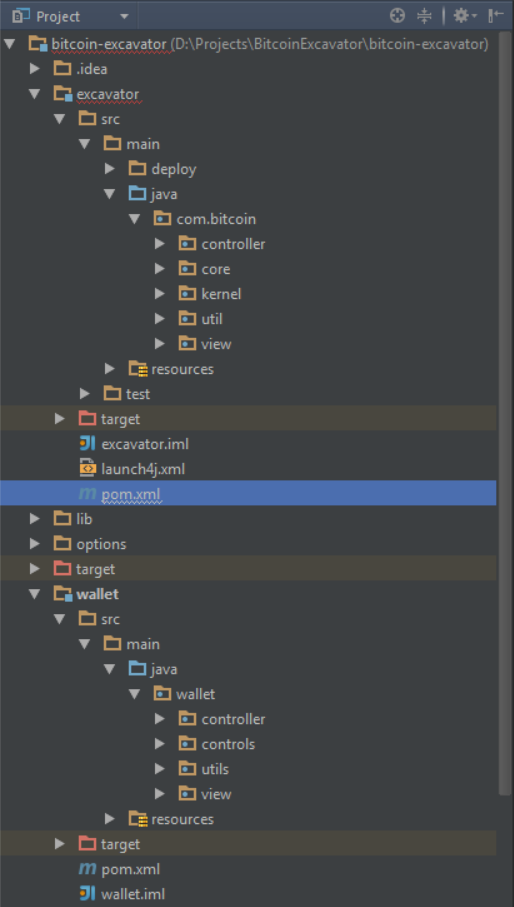
\includegraphics{images/project_structure.PNG}

\subsection{Technologie}

Projekt napisano w języku Java, wykorzystując system zarządzania projektem Maven.

Kod OpenCL uruchamiano przy użyciu gotowej biblioteki kompilującej.
Fundamenty związane z komunikacją sieciową w ramach przetwarzania bitcoinów zrealizowane zostały w wykorzystanej przez nas bibliotece BitcoinJ.

Dla stworzenia interfejsu graficznego wykorzystano bibliotekę JavaFX.
Mniej istotnymi bibliotekami również przez nas wykorzystanymi są Apache Commons (klasy i metody pomocnicze), log4j (system logowania zdarzeń),  json-io (zapis opcji na dysk).

\subsection{Kod kernela}

\begingroup
    \fontsize{7pt}{10pt}\selectfont
    \begin{verbatim}
    /*
 * BitCoin Excavator - OpenCL miner for BitCoin
 *
 * This program is free software: you can redistribute it and/or modify
 * it under the terms of the GNU General Public License as published by
 * the Free Software Foundation, either version 3 of the License, or
 * (at your option) any later version.
 *
 * This program is distributed in the hope that it will be useful,
 * but WITHOUT ANY WARRANTY; without even the implied warranty of
 * MERCHANTABILITY or FITNESS FOR A PARTICULAR PURPOSE.	See the
 * GNU General Public License for more detail).
 *
 * You should have received a copy of the GNU General Public License
 * along with this program.	If not, see <http://www.gnu.org/licenses/>.
 */

typedef uint z;

#if BITALIGN
#pragma OPENCL EXTENSION cl_amd_media_ops : enable
#define Zrotr(a, b) amd_bitalign((z)a, (z)a, (z)(32 - b))
#else
#define Zrotr(a, b) rotate((z)a, (z)b)
#endif

#if BFIINT
#define ZCh(a, b, c) amd_bytealign(a, b, c)
#define ZMa(a, b, c) amd_bytealign((c ^ a), (b), (a))
#else
#define ZCh(a, b, c) bitselect((z)c, (z)b, (z)a)
#define ZMa(a, b, c) bitselect((z)a, (z)b, (z)c ^ (z)a)
#endif

#define ZR25(n) ((Zrotr((n), 25) ^ Zrotr((n), 14) ^ ((n) >> 3U)))
#define ZR15(n) ((Zrotr((n), 15) ^ Zrotr((n), 13) ^ ((n) >> 10U)))
#define ZR26(n) ((Zrotr((n), 26) ^ Zrotr((n), 21) ^ Zrotr((n), 7)))
#define ZR30(n) ((Zrotr((n), 30) ^ Zrotr((n), 19) ^ Zrotr((n), 10)))

__kernel __attribute__((reqd_work_group_size(WORKSIZE, 1, 1))) void search(
	const uint PreVal4_state0, const uint PreVal4_state0_k7,
	const uint PreVal4_T1,
	const uint W18, const uint W19,
	const uint W16, const uint W17,
	const uint W16_plus_K16, const uint W17_plus_K17,
	const uint W31, const uint W32,
	const uint d1, const uint b1, const uint c1,
	const uint h1, const uint f1, const uint g1,
	const uint c1_plus_k5, const uint b1_plus_k6,
	const uint state0, const uint state1, const uint state2, const uint state3,
	const uint state4, const uint state5, const uint state6, const uint state7,
	__global uint * output)
{
	z ZA[930];

	uint noncebase = get_global_id(0);

	z Znonce = noncebase;
	uintzz nonce = (uintzz)0;

	ZA[15] = Znonce + PreVal4_state0;

	ZA[16] = (ZCh(ZA[15], b1, c1) + d1) + ZR26(ZA[15]);
	ZA[26] = Znonce + PreVal4_T1;

	ZA[27] = ZMa(f1, g1, ZA[26]) + ZR30(ZA[26]);
	ZA[17] = ZA[16] + h1;

	ZA[19] = (ZCh(ZA[17], ZA[15], b1) + c1_plus_k5) + ZR26(ZA[17]);
	ZA[28] = ZA[27] + ZA[16];

	ZA[548] = ZMa(ZA[26], f1, ZA[28]) + ZR30(ZA[28]);
	ZA[20] = ZA[19] + g1;

	ZA[22] = (ZCh(ZA[20], ZA[17], ZA[15]) + b1_plus_k6) + ZR26(ZA[20]);
	ZA[29] = ZA[548] + ZA[19];

	ZA[549] = ZMa(ZA[28], ZA[26], ZA[29]) + ZR30(ZA[29]);
	ZA[23] = ZA[22] + f1;

	ZA[24] = ZCh(ZA[23], ZA[20], ZA[17]) + ZR26(ZA[23]);
	ZA[180] = Znonce + PreVal4_state0_k7;
	ZA[30] = ZA[549] + ZA[22];

	ZA[31] = ZMa(ZA[29], ZA[28], ZA[30]) + ZR30(ZA[30]);
	ZA[181] = ZA[180] + ZA[24];

	ZA[182] = ZA[181] + ZA[26];
	ZA[183] = ZA[181] + ZA[31];
	ZA[18] = ZA[17] + 0xd807aa98U;
	
[...]

	ZA[918] = (ZCh(ZA[914], ZA[909], ZA[904]) + ZA[917]) + ZR26(ZA[914]);
	ZA[915] = ZMa(ZA[906], ZA[901], ZA[911]) + ZR30(ZA[911]);
	ZA[733] = ZR15(ZA[727]) + ZA[732];
	ZA[919] = ZA[906] + ZA[904] + ZA[731];
	ZA[734] = ZA[712] + ZA[681];

	ZA[920] = (ZCh(ZA[918], ZA[914], ZA[909]) + ZA[919]) + ZR26(ZA[918]);
	ZA[735] = ZR15(ZA[730]) + ZA[734];
	ZA[921] = ZA[911] + ZA[909] + ZA[733];
	ZA[916] = ZA[913] + ZA[915];

	ZA[922] = (ZCh(ZA[920], ZA[918], ZA[914]) + ZA[921]) + ZR26(ZA[920]);
	ZA[923] = ZA[916] + ZA[914] + ZA[735];

	ZA[924] = (ZCh(ZA[922], ZA[920], ZA[918]) + ZA[923]) + ZR26(ZA[922]);

	bool Zio = any(ZA[924] == (z)0x136032EDU);

	bool io = false;
	io = (Zio) ? Zio : io;

	nonce = (io) ? Znonce : nonce;

	if(io) { output[0] = (uintzz)nonce; }
}

// vim: set ft=c
    \end{verbatim}  
\endgroup

\subsection{Interfejs}

Na interfejs graficzny projektu składają się widoku dwóch połączonych ze sobą aplikacji: koparki i portfela.

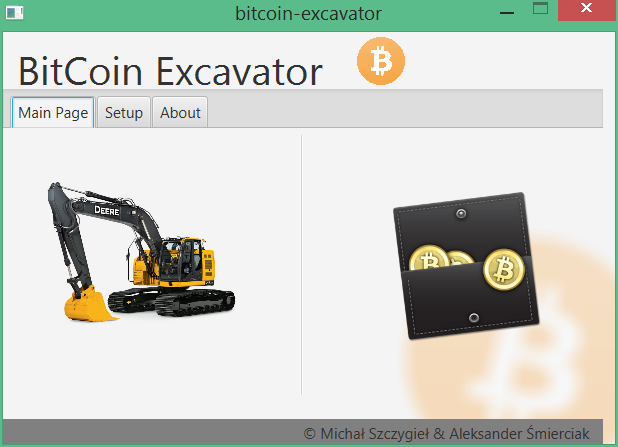
\includegraphics[width=10cm]{images/excavator_main_screen.PNG}

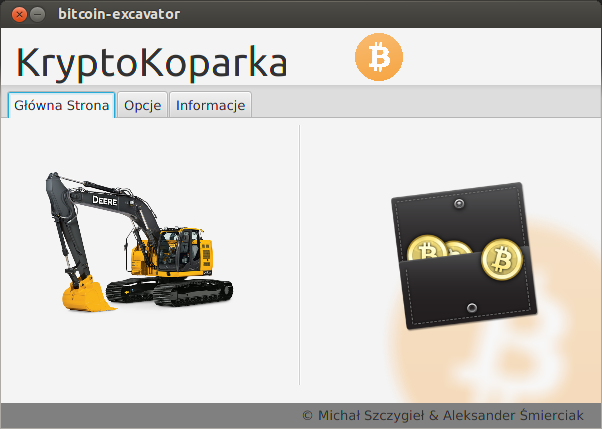
\includegraphics[width=10cm]{images/excavator_main_screen_ubuntu.PNG}

Przy pomocy koparki można:
\begin{enumerate}
 \item skonfigurować sposób łączenia się z siecią Bitcoin i wykorzystania karty graficznej sprzętu
 
        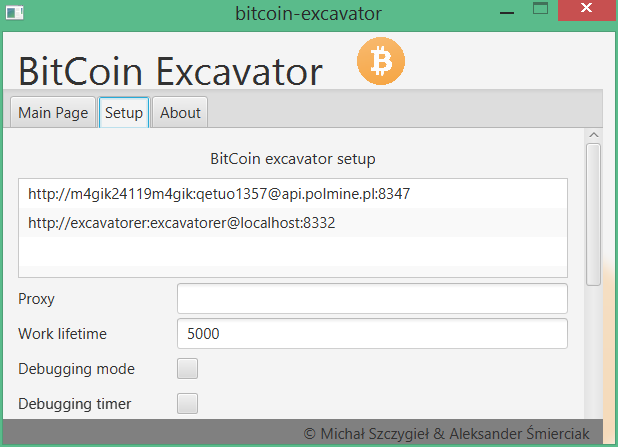
\includegraphics[width=10cm]{images/excavator_options_screen.PNG}
 \item uruchomić lub zatrzymać proces kopania
\end{enumerate}

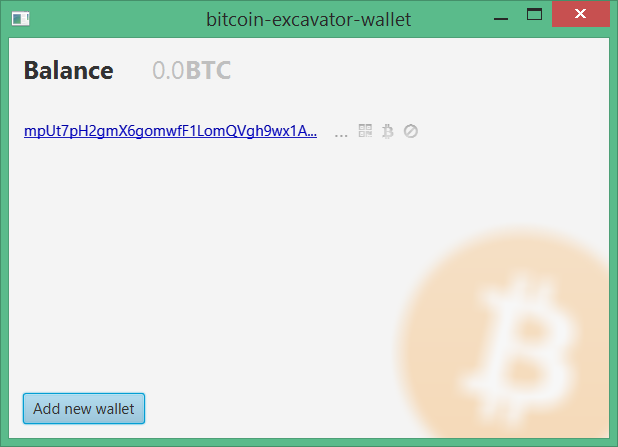
\includegraphics[width=10cm]{images/wallet_main_screen.PNG}

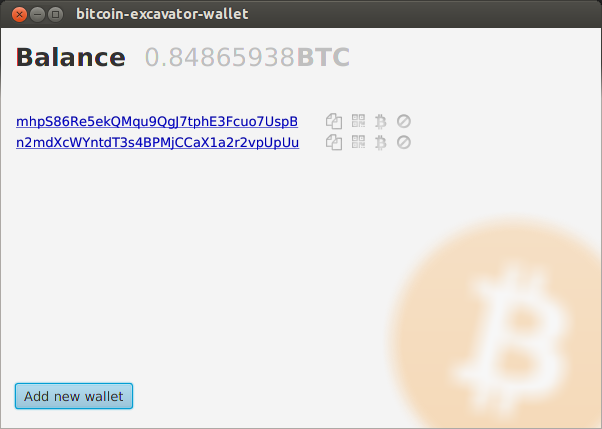
\includegraphics[width=10cm]{images/wallet_main_screen_ubuntu.PNG}

Przy pomocy portfela można:
\begin{enumerate}
 \item sprawdzić stan swojego portfela
 \item wysłać pieniądze do zdefiniowanego hashem portfela
 
       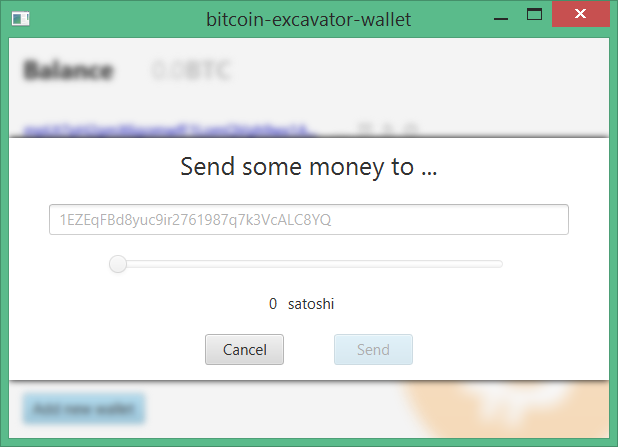
\includegraphics[width=10cm]{images/wallet_send_screen.PNG}
 \item pobrać sam adres lub kod QR adresu swojego portfela do schowka
 
       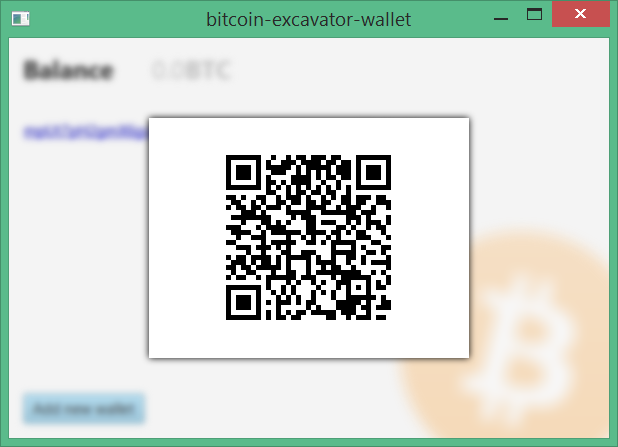
\includegraphics[width=10cm]{images/wallet_qr_screen.PNG}
 \item dodać lub usunąć portfel z aplikacji
 
       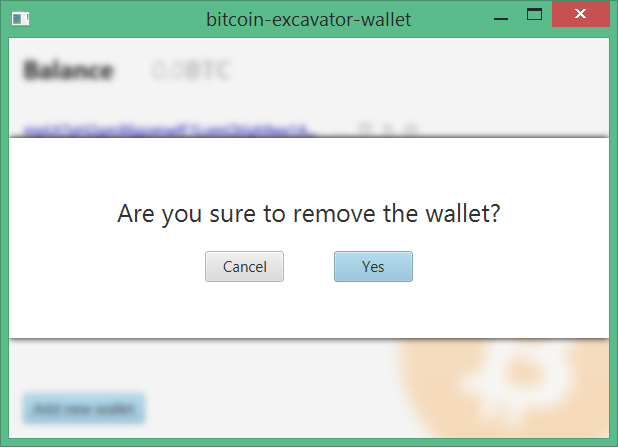
\includegraphics[width=10cm]{images/wallet_remove_screen.PNG}
\end{enumerate}

\subsection{Proces realizacji}

Współpracę nad projektem z programistycznego punktu widzenia ułatwił serwis GitHub, dostarczający repozytoria systemu kontroli wersji Git.
Prace nad projektem można przeglądnąć pod adresem
https://github.com/M4GiK/BitcoinExcavator

\subsection{Rezultat pracy}

Rezultatem pracy jest aplikacja która spełnia wszystkie postawione na początku w specyfikacji wymagania i która pozwala na pełnoprawne uczestnictwo w przetwarzaniu bitcoinów.

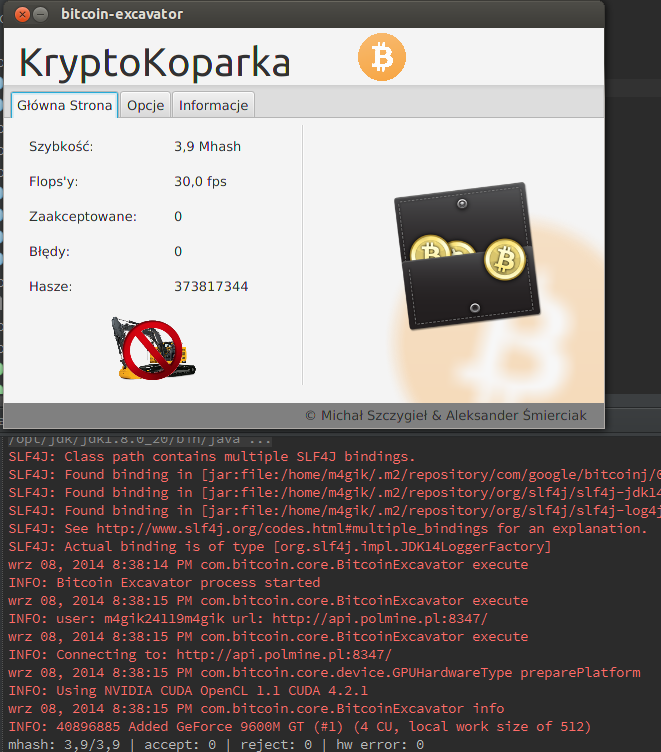
\includegraphics[width=10cm]{images/excavator_digging_screen_ubuntu.PNG}

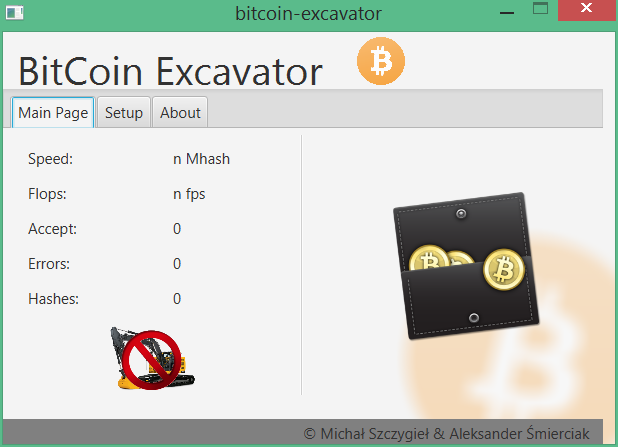
\includegraphics[width=10cm]{images/excavator_digging_error_screen.PNG}

Projekt ten dostarczył nam możliwość poznania bliżej sposobu działania tej konkretnej kryptowaluty, a także ogólnego mechanizmu stojącego za kryptowalutami.

\subsection{Literatura}

\begin{enumerate}
  \item \url{http://enetium.com/resources/Bitcoin.pdf}
  \item \url{https://bitcoin.org/en/bitcoin-for-developers}
  \item \url{https://github.com/gavinandresen/bitcointools/blob/master/NOTES.txt}
  \item \url{https://bitcoin.org/en/developer-documentation}
  \item \url{https://bitcoin.org/bitcoin.pdf}
  \item \url{https://en.bitcoin.it/wiki/Protocol_rulesa}
  \item \url{https://en.bitcoin.it/wiki/Category:Technical}
\end{enumerate}

\end{document}